\documentclass{article}

% Package necessari
\usepackage{geometry}
\usepackage[utf8]{inputenc}
\usepackage[english]{babel}
\usepackage[sfdefault]{roboto}
\usepackage[T1]{fontenc}
\usepackage[font={small,sl}]{caption}
\usepackage[font={small,sl}]{subcaption}
\usepackage{graphicx}
\usepackage[usenames, table, dvipsnames]{xcolor}
\usepackage{hyperref}
\usepackage[most]{tcolorbox}
\usepackage[section]{placeins}
\usepackage{soulutf8}
\usepackage{listings}
\usepackage{tabularray}
\usepackage{amssymb}

% Impostazione dei margini
\geometry{
	a4paper,
	left=20 mm,
	top=20 mm,
	bottom=20 mm,
	right=20 mm,
}

% Titolo del documento
\title{\small Report of "Network \& System defense" project \\
\Huge \textbf{MLKM SHIELD}\\
\Large (Protection against malicious LKM)}

% Autore del documento
\author{Simone Tiberi (M. 0299908)\\%
email: \texttt{\href{mailto:simone.tiberi.98@gmail.com}{simone.tiberi.98@gmail.com}}}

% Data del documento
\date{\today}

% Impostazione delle lunghezze di alcuni elementi del documento
\setlength{\parskip}{1em}
\setlength{\parindent}{0em}

% Impostazioni del package hyperref
\hypersetup{
        colorlinks=true,
        linktocpage=true,
        linkcolor=blue,
        urlcolor=blue,
        citecolor=blue,
        pdftitle={NSD project report},
        pdfauthor={Simone Tiberi},
}

% Tokyonight colors
\definecolor{tn-bg}{HTML}{24283b}
\definecolor{tn-terminal}{HTML}{414868}
\definecolor{tn-red}{HTML}{f7768e}
\definecolor{tn-fg}{HTML}{c0caf5}
\definecolor{tn-fg-dark}{HTML}{a9b1d6}
\definecolor{tn-green}{HTML}{9ece6a}
\definecolor{tn-comment}{HTML}{565f89}
\definecolor{tn-blue0}{HTML}{3d59a1}
\definecolor{tn-blue}{HTML}{7aa2f7}
\definecolor{tn-cyan}{HTML}{7dcfff}

% Impostazioni listings
\lstset{
	language=C,
	frame=shadowbox,
    backgroundcolor=\color{tn-bg},
	rulesepcolor=\color{tn-terminal},
    basicstyle=\color{tn-fg}\ttfamily\scriptsize,
	keywordstyle=\color{tn-red}\bfseries\scriptsize,
	stringstyle=\color{tn-green}\scriptsize,
	commentstyle=\color{tn-comment}\scriptsize,
	numbers=left,
	numberstyle=\tiny\color{tn-fg-dark},
	numbersep=5pt,
	tabsize=2,
	showtabs=false,
	showspaces=false,
	showstringspaces=false,
	escapechar=|,
	captionpos=b,
	breaklines=true,
	keepspaces=true
}

\lstdefinelanguage{diff}{
	basicstyle=\color{tn-fg}\ttfamily\scriptsize,
	morecomment=[f][\color{tn-comment}\scriptsize]{@@},
	morecomment=[f][\color{tn-green}\scriptsize]{+\ },
	morecomment=[f][\color{tn-red}\scriptsize]{-\ },
}

% Cartella di default delle immagini
\graphicspath{ {./figs/} }

% Impostazioni della colorbox
\newtcolorbox{custombox}[2]{%
	colback=white,
	colframe=#2,
	colbacktitle=white!90!#2,
	coltitle=black,
	fonttitle=\bfseries,
	fontupper=\small,
	title=#1,
	enhanced,
	left=2pt, right=2pt, top=8pt, bottom=2pt,
	attach boxed title to top center={yshift=-3mm}
}

% Non mostrare le sotto-sezioni nella tavola dei contenuti
\setcounter{tocdepth}{2}

% Comando utile per "mostrare una shell" nel documento (e.g. per i comandi)
\newcommand{\terminal}[1]{\colorbox{tn-bg}{\textcolor{tn-fg}{\texttt{#1}}}}

\begin{document}
	\maketitle
	\tableofcontents
	\newpage

	\section{Project specification}
	This project entails writing some protection mechanism in the Linux kernel (as a patch, a security module, a simple
	module, \dots) to prevent malicious loadable kernel modules to tamper with internal data structures of the kernel.

	In particular, beyond the example that we have discussed in class, it is possible that a module will not perform
	any attack during the loading phase, but it will perform some form of delayed attack (e.g., by relying on a
	Tasklet). Your scheme should also be able to perform this kind of detection.

	If a module is detected as malicious, it must be unmounted, and any possible side effect generated by it should be
	reverted.

	\section{Project structure}
	\begin{custombox}{Repository}{blue}
		Link to Github repository: \url{https://github.com/tibwere/mlkm-shield}
	\end{custombox}

	The code base is divided into several files, each of which contains stuffs relating to certain components of the
	project (e.g. hooks, \textit{machine-specific} operations, \dots).

	The following sections are aimed at describing each of them, by analyzing core data structures and procedures
	implemented, as well as the general idea behind the functioning of the module.

	\section{Introduction to LKM monitoring}
	The protection mechanism is based on the following assumptions:
	\begin{enumerate}
		\item when the shield module is mounted, the memory is in a \textit{good} state. This is reasonable, otherwise
		it would be impossible to protect the system.

		Because of this, in the beginning of the installation process the state of the critical memory areas is cached;

		\item the areas to be protected are immutable over the time and therefore it is not necessary to update the
		caching status \textit{continuously}. This is reasonable too, especially for memory areas like system call
		table and \texttt{IDT};

		\item any module not monitored by the shield does not make any changes in critical memory areas.
	\end{enumerate}


	The areas considered critical and therefore monitored by the shield module are:
	\begin{itemize}
		\item \textbf{System call table}, because a rootkit can change some function pointers within the table and thus
		change the behavior of certain system calls;
		\item \textbf{IDT} (\textbf{I}nterrupt \textbf{D}escriptor \textbf{T}able), because a rootkit can modify
		interrupt handlers to perform malicious activity;
		\item a list of \textbf{additional symbols} (e.g. some crypto keys) that the sysadmin can specify inside a
		configuration file (sec.~\ref{sec:config}) before mounting the shield module.
	\end{itemize}

	Taking advantage of the \texttt{kretpobe} (and also \texttt{kprobe}) mechanisms offered by Linux
	Kernel, the very last function invoked inside the mounting process is hooked, so
	that after the return statement, a \textbf{verification step} can begin (fig.~\ref{fig:monitoring}).

	\begin{figure}[!htbp]
		\centering
		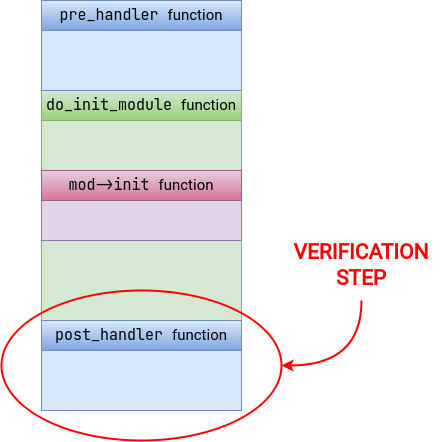
\includegraphics[scale=0.4]{monitoring}
		\caption{Hook scheme for \texttt{do\_init\_module}}
		\label{fig:monitoring}
	\end{figure}

	Obviously, using only this mechanism, a condition like the following one could occur:
	\begin{itemize}
		\item a non-malicious module $A$ is running a function $\alpha$,
		\item a malicious module $B$ is running \textbf{concurrently} (such as shown in fig.~\ref{fig:concurrency}) a
		function $\beta$,
		\item the shield module recognize $A$ as malicious and also $B$ as non-malicious thus \textbf{making two
		mistakes}.
	\end{itemize}

	\begin{figure}[!htbp]
		\centering
		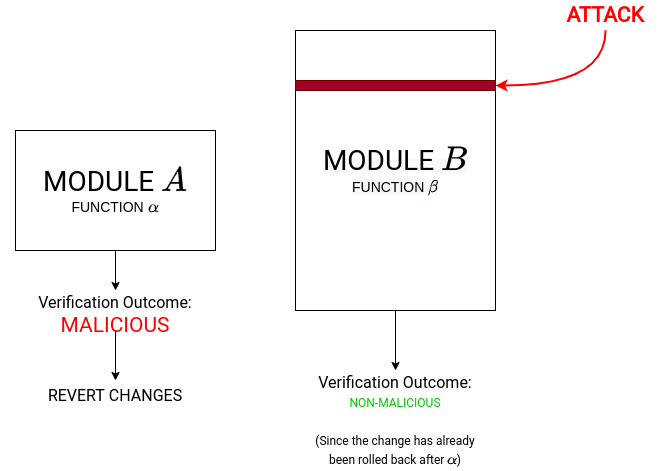
\includegraphics[scale=0.4]{concurrency}
		\caption{Detection scheme problem without using a \textit{barrier}}
		\label{fig:concurrency}
	\end{figure}

	For this reason the use of a \textit{barrier} was introduced. The idea is the following:
	\begin{enumerate}
		\item in the \textbf{pre-handler} the thread that is mounting the module, try to acquire a \texttt{spin\_lock}
		before do it,
		\item in the \textbf{post-handler} the thread release the lock allowing other monitored modules to progress in
		the execution of their activities.
	\end{enumerate}

	This mechanism ensures that no other monitored module can interfere, but obviously it causes an inevitable
	performance degradation due to the introduction of a synchronization mechanism.

	Finally, for the detection of malicious actions in deferred mode, the probe mechanism was exploited again in the
	same way, this time dynamically hooking functions inside the modules, as described in detail in
	section~\ref{sec:hooks}.

	\section{Components description}

	\subsection{\emph{Black/White list} component}\label{sec:bwlist}
	This component simply contains a function and a couple of macros for inserting modules into the black/white list.
	These two lists allow to realize the following mechanisms:
	\begin{itemize}
		\item a module present in the \textbf{white list} is considered \textit{a priori} not malicious and therefore
		is not subject to monitoring, which implies that it will not be damaged in terms of performance, due to the use
		of kretprobes and spinlocks,
		\item a module present in the \textbf{black list} is considered \textit{a priori} malicious and therefore is
		removed directly. In section~\ref{sec:hooks} it will be showed the mechanism used to safely remove this kind of
		module without risking the execution of malicious code.
	\end{itemize}

	\subsection{\emph{Configuration} component}\label{sec:config}
	Some variables are defined in this component that a sysadmin can change, before the installation of the
	shield, to tune it according to their needs. In particular there are:
	\begin{itemize}
		\item two boolean variables to decide whether or not to secure system call table and \texttt{IDT} respectively;
		\item the list of additional symbols to protect, where you do not have to specify the address directly,
		but the name of the symbol, readable from \texttt{/proc/kallysms};
		\item the modules inside the white and the black list.
	\end{itemize}

	\subsection{\emph{Hooks} component}\label{sec:hooks}
	This is the most complex component in the module. For this reason the analysis is divided into subsections as
	follows.

	\subsubsection{Kretprobe hooked to \texttt{do\_init\_module}}
	This probe mechanism makes use of dedicated data structures (list.~\ref{lst:krp-data}):
	\begin{itemize}
		\item the enumeration \texttt{post\_do\_init\_module\_activities}, which contains all possible activities that
		the pre-handler can schedule to do for the post-handler;
		\item the structure \texttt{krp\_do\_init\_module\_data}, which contains elements that must be passed from the
		pre-handler to the post one.
	\end{itemize}


	The pre-handler of \texttt{do\_init\_module} function is \texttt{start\_monitoring\_module} in which:
	\begin{enumerate}
		\item the address of the \texttt{module} structure (1$^{\text{st}}$ parameter) is retrieved using
		\texttt{regs\_get\_kernel\_argument} instead of accessing directly \texttt{RDI} register to enhance
		portability of the code;
		\item it is checked if the module belongs to the white list and if so, the remaining part is skipped
		and the function return immediately\footnote{It should be noted that returning a value other than \texttt{0}
		(e.g. \texttt{-EINVAL}), the post handler is not activated.};
		\item it is checked if the module belongs to the black list and if so, it is invalidated and the function
		returns immediately;
		\item the structure \texttt{monitored\_module} (sec~\ref{sec:shield}) is initialized;
		\item all the functions inside the module are hooked up, by making an ELF inspection. If this activity were
		carried out in the post handler	a scenario like the following one would be possible:
		\begin{enumerate}
			\item in the \texttt{mod->init} function the malicious module schedule a deferred work
			\item this one starts to execute, \textbf{before} the kretprobe is attached
		\end{enumerate}

		\begin{custombox}{Pay attention}{Goldenrod}
			If the
			\href{https://elixir.bootlin.com/linux/v5.17/source/include/asm-generic/kprobes.h#L15}{\texttt{NOKPROBE\_SYMBOL}}
			macro is applied to a function within the module, this could not be fully monitored, so it is judged
			to be malicious.
		\end{custombox}
		\item the barrier is acquired, and finally the module is added to the \texttt{monitored\_modules\_list}.
	\end{enumerate}

	To invalidate a module, the \texttt{krp\_do\_init\_module\_data} structure is used. In particular, depending on the
	value of the \texttt{what\_to\_do} member, the pointer enclosed in the \texttt{union} assumes a different semantics:
	\begin{itemize}
		\item if \texttt{what\_to\_do} is \texttt{REMOVE\_MODULE}, therefore the pointer is a \texttt{struct module *};
		\item otherwise the pointer is \texttt{struct monitored module *}.
	\end{itemize}

	By the way, if the \texttt{mod->init} function is executed, an hack on critical memory area could occur. To avoid
	that, in the \texttt{invalid[\_monitored]\_module} macros, the pointers to \texttt{init} and \texttt{exit} function
	are updated to point to dummy functions defined into the shield module.

	The behavior of the post-handler (function \texttt{verify\_after\_module\_installation}) is driven by the value of
	the \texttt{what\_to\_to} member:
	\begin{itemize}
		\item if \texttt{REMOVE\_MODULE}, then the \texttt{free\_module} function is invoked on the pointer to
		\texttt{struct module};
		\item else, if \texttt{REMOVE\_MONITORED\_MODULE} then the \texttt{remove\_malicious\_lkm} function
		(sec.~\ref{sec:shield}) is invoked on the \texttt{struct monitored\_module} pointer;
		\item else (\texttt{DONT\_REMOVE}) the \texttt{verify\_safe\_area} function (sec~\ref{sec:safemem}) is invoked
		and in case of threat detected, \texttt{remove\_malicious\_lkm} is invoked.
	\end{itemize}

	In any case in the very end of the function, the barrier is released.

	\subsubsection{Kretprobe hooked to functions inside monitored modules}
	Every function inside a monitored module is hooked up with a kretprobe such that:
	\begin{itemize}
		\item in the \textbf{pre-handler} simply nested verification are avoided by checking \texttt{under\_analysis}
		flag and then an attempt is made to acquire the lock;
		\item in the \textbf{post-handler}, \texttt{verify\_safe\_area} is invoked and in case of threat
		detected, \texttt{remove\_malicious\_lkm} is invoked.
	\end{itemize}

	\subsubsection{Kprobe hooked to \texttt{free\_module}}
	Obviously all kretprobes dynamically hooked to functions inside monitored module need to be unregistered when the
	module is unmounted (because a threat has found or simply because someone has invoked \texttt{rmmod} on it).

	For this reason, a kprobe is hooked to the \texttt{free\_module} function and in the pre-handler, if the
	module to be freed is currently monitored, it is cleaned up and removed from the list.

	\subsection{\emph{Module} component}\label{sec:module}
	This component simply defines \texttt{init} and \texttt{cleanup} functions and also some elements for module
	management (e.g. \texttt{module\_param}, \texttt{MODULE\_LICENSE}, \dots).

	\subsection{\emph{Safe memory} component}\label{sec:safemem}
	This is one of the core components of the module. Inside of it, it is defined the data structure
	\texttt{safe\_area} (list.~\ref{lst:safe-area}), which is the logical representation for the caching of	a specific
	\textit{quad word} (\texttt{64 bits}) in memory.

	Inside the module three different arrays of \texttt{safe\_area} structures are used:
	\begin{itemize}
		\item one for system call table function pointers, of size \texttt{NR\_syscalls};
		\item one for \texttt{IDT}, seen as a sequence of \texttt{unsigned long}, which implies that the size of array
		is evaluated as:
		\begin{equation*}
			\dfrac{\mathtt{IDT\_ENTRIES} \cdot \mathtt{sizeof(gate\_desc)}}{\mathtt{sizeof(unsigned\ long)}}
		\end{equation*}
		\item one for the list of additional symbols specified inside the array in the configuration file.
	\end{itemize}

	One of the main functions defined in this component is \texttt{verify\_safe\_areas} used in some handlers defined
	into the \emph{hooks} component. Inside of it, the function \texttt{inspect\_sa} is called for each array to check
	if critical memory areas have been altered. In this case:

	\begin{itemize}
		\item a new threat is added to the \texttt{/sys} audit (sec.~\ref{sec:threats});
		\item the hacked memory area is restored, after disabling the memory protection by overwriting the \texttt{CR0}
		register (sec~\ref{sec:x86}).
	\end{itemize}

	\subsection{\emph{Shield} component}\label{sec:shield}
	Inside this component are defined two core structures for the functionality of the module:
	\begin{itemize}
		\item \texttt{monitored\_module}, which contains metadata used to monitor the module, such as the reference to
		the \texttt{struct module}, a boolean value used to avoid nested verifications, and two set of pointers used to
		realize two different linked lists:
		\begin{itemize}
			\item the former, links together all monitored modules;
			\item the latter, links a monitored module to the kretprobes hooked to its own functions.
		\end{itemize}

		\item \texttt{module\_probe}, which represents a \texttt{kretprobe} hooked to a specific function of the module,
		so inside of it there are the reference to the owner (\texttt{struct monitored\_module *}), the
		\texttt{kretprobe} itself and finally a couple of pointers used to link all the probes related to the same
		module together and to the owner too.
	\end{itemize}

	In list.~\ref{lst:shield-structs} are shown these structures and furthermore in fig.~\ref{fig:shield-structs} is
	represented how they are linked together.

	\begin{figure}[!htbp]
		\centering
		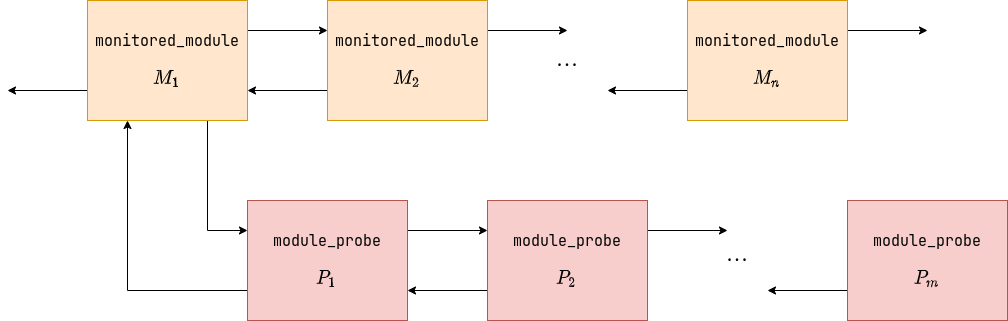
\includegraphics[scale=0.4]{shield-structs}
		\caption{Relationship between \texttt{monitored\_module} and \texttt{module\_probe}}
		\label{fig:shield-structs}
	\end{figure}

	Inside this component is defined also a parameter of the module, that is the \texttt{removed} variable. At any time
	is it possible to see how many modules have been detected as malicious reading the content of the pseudo-file
	\texttt{/sys/module/mlkm\_shield/parameters/removed}.

	An interesting function defined inside this module is \texttt{remove\_malicious\_lkm}. To remove a module you need
	to use the function \texttt{free\_module}, which is not exported by default for module programming. For this
	reason, its address has been retrieved using a function defined inside the \textbf{symbols} component
	(sec.~\ref{sec:symbols}).

	\subsection{\emph{Symbols} component}\label{sec:symbols}
	In this component are defined some utility functions used by other ones, such as:
	\begin{itemize}
		\item \texttt{symbol\_lookup}, which allows you to retrieve the address of a symbol in the kernel memory space
		specifying its name. To do this you need to use the \texttt{kallsyms\_lookup\_name} function, which is no
		longer available for module programming starting with kernel 5.7, so the kprobing mechanism was used to
		retrieve its address;
		\item \texttt{get\_system\_call\_table\_address}, which by relying on the previous one, lets you to retrieve
		the address of the system call table. Up to version 4.4 of Linux, the search is carried out according to a
		brute force approach, starting from the address of \texttt{the sys\_close} system call\footnote{For
			conventional Linux Kernel builds, this address is lower than the system call table one.};
		\item \texttt{get\_idt\_address}, which allows you to retrieve the base address of the \texttt{IDT}, by relying
		on the \texttt{SIDT} instruction wrapped into the
		\href{https://elixir.bootlin.com/linux/latest/source/arch/x86/include/asm/desc.h#L223}{\texttt{store\_idt}} API
		of the kernel.
	\end{itemize}

	\subsection{\emph{Threat audit on \texttt{sysfs}} component}\label{sec:threats}
	This component realizes an additional feature for the module. The idea is to provide an easier way to know if some
	threats are detected, instead of analyze \texttt{dmesg} output. This is exploited using the pseudo-file in
	\texttt{sysfs}:

	\centerline{\texttt{/sys/kernel/mlkm\_shield/threats}}

	\begin{figure}[!htbp]
		\centering
		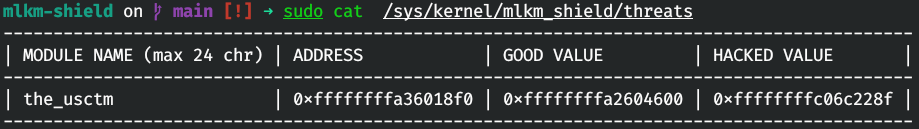
\includegraphics[scale=0.4]{threats}
		\caption{Output of \texttt{/sys/kernel/mlkm\_shield/threats}}
		\label{fig:threats}
	\end{figure}

	To do this, first of all it is defined a structure \texttt{threat} in which are contained all information printed
	out in this pseudo-file (list.~\ref{lst:threats}).

	Every time that a threat is detected, \texttt{insert\_new\_threat} is invoked to add an instance of \texttt{struct
	threat} to the list. Since the insertion needs to be synchronized, if it happened along the thread that is
	verifying, it would cause a block which could be unwanted. For this reason, the workqueue mechanism is exploited by
	declaring the \texttt{threats-sys-audit} single-threaded queue (to maintain the FIFO ordering) and inserting the
	request for addition in it.

	\subsection{\emph{Machine specific (x86)} component}\label{sec:x86}
	This component simply contains a function and a couple of macros to modify \texttt{CR0} register to enable/disable
	memory protection. For all this, the bit \texttt{X86\_CR0\_WP} is changed using \texttt{memory} clobber to avoid
	compile-time instruction reordering (according to
	\href{https://elixir.bootlin.com/linux/v5.17.3/source/arch/x86/include/asm/special_insns.h#L54}{this}
	implementation).

	As you can see by analyzing the source code, the module uses machine-specific facilities for x86, so for a possible
	porting to other architectures it would be necessary to define additional header files in the \texttt{asm}
	directory and different implementations of the API C using \texttt{\#define CONFIG\_XXX} directives.

	\section{Module installation}
	To install \texttt{mlkm\_shield} module it is possible to exploit rules specified inside the \texttt{Makefile}:
	\begin{itemize}
		\item \terminal{\$ make} to build the module, using the \texttt{make modules} rule of \texttt{Kbuild};
		\item \terminal{\# make install} to mount the module, using \texttt{/sbin/insmod} command;
		\item \terminal{\$ make clean} to cleanup the build output from the local working directory;
		\item \terminal{\# make clean-all}, in addition to the previous one, to unmount the module
		using \texttt{/sbin/rmmod} command if this is actually mounted, using a conditional construct to avoid
		errors.
	\end{itemize}

	\section{Tests carried out}
	The tab.~\ref{table:machines} summarizes the specifications of the machines used to test the module.

	\begin{table}[htbp]
		\centering
		\begin{tblr}{
				colspec = {|l|l|l|l|l|},
				hlines,
				row{odd} = {tn-blue!80, font=\footnotesize},
				row{even} = {tn-cyan!80, font=\footnotesize},
				row{1} = {tn-blue0!80,font=\footnotesize\color{white}},
			}
			Machine & Linux distribution & Kernel version & Processors & Memory \\
			Physical & Arch Linux (x86\_64) & 5.15.37-1-lts & i5-5300U (4) @ 2.900GHz & 16 MB \\
			Virtual & Ubuntu 20.04.4 LTS (x86\_64) & 5.13.0-39-generic & i5-5300U (2) @ 2.294GHz & 4 MB \\
		\end{tblr}
		\caption{Characteristics of the machines used for testing}
		\label{table:machines}
	\end{table}


	As you can see in tab.~\ref{table:pc}, a performance comparison was made using the physical machine. The test aims
	to show the overhead impact of the shield on the mount/unmount phase of other modules. In this regard, a
	deliberately simple module (list.~\ref{lst:dummy}) was used, to evaluate the performance of the mount
	(\textit{resp. unmount}) process in a more isolated way without the influence of the overhead of the
	\texttt{mod->init} (\textit{resp. \texttt{mod->exit}}) itself.

	\begin{table}[htbp]
		\centering
		\begin{tblr}{
				colspec = {|l|l|l|},
				hlines,
				row{odd} = {tn-blue!80, font=\footnotesize},
				row{even} = {tn-cyan!80, font=\footnotesize},
				row{1} = {tn-blue0!80,font=\footnotesize\color{white}},
			}
			\texttt{mlkm\_shield} & \texttt{insmod} & \texttt{rmmod} \\
			Not mounted & 0,004 s & 0,043s \\
			Mounted & 0,154 s & 0,262 s \\
		\end{tblr}
		\caption{Performance comparison}
		\label{table:pc}
	\end{table}

	Furthermore, tab.~\ref{table:tests} shows a list of modules on which the shield has been tested and the result
	obtained.

	\begin{table}[htbp]
		\centering
		\begin{tblr}{
				colspec = {|l|l|l|l|c|},
				hlines,
				row{odd} = {tn-blue!80, font=\footnotesize},
				row{even} = {tn-cyan!80, font=\footnotesize},
				row{1} = {tn-blue0!80,font=\footnotesize\color{white}},
			}
			Module & Outcome & Reason & Notes & Status\\
			\texttt{rootkit} & {\color{red}\textbf{removed}} & a function is not hookable & example module discussed in
			class & \textbf{\color{ForestGreen}\checkmark}\\
			\texttt{the\_usctm} & {\color{red}\textbf{removed}} & a critical area changed & Github
			\href{https://github.com/FrancescoQuaglia/Linux-sys_call_table-discoverer}{link} &
			\textbf{\color{ForestGreen}\checkmark}\\
			\texttt{the\_tasklet\_usctm} & {\color{red}\textbf{removed}} & a critical area changed & patch of the
			original \texttt{the\_usctm} (list.~\ref{lst:tasklet-usctm}) & \textbf{\color{ForestGreen}\checkmark}\\
			\texttt{dummy\_module} & {\color{ForestGreen}\textbf{not removed}} & the LKM is not malicious & module
			written by me (list.~\ref{lst:dummy}) & \textbf{\color{ForestGreen}\checkmark}\\
			\texttt{symbol\_finder} & {\color{ForestGreen}\textbf{not removed}} & the LKM is not malicious & module
			written by me (list.~\ref{lst:symbfnd}) & \textbf{\color{ForestGreen}\checkmark}\\
		\end{tblr}
		\caption{Tests carried out}
		\label{table:tests}
	\end{table}

	\section{Future development}
	Some ideas to enhance the possibilities of this module to detect malicious LKM are shown below:
	\begin{itemize}
		\item calculate and cache the hash of the body of each system call/interrupt handler to eventually identify hot
		patching attempts;
		\item cache the status of some fields of the module structure (e.g. \texttt{sect\_attrs}) and then check if
		they remain unchanged after execution of \texttt{mod->init};
		\item verify if the module remove itself from the linked list, because this can be a sign that it is
		malicious (\textit{why a module needs to hide itself?}).
	\end{itemize}

	\section{Source codes mentioned in the document}
	\lstinputlisting[
		caption={Data types and structures defined inside \emph{hook} component},
		label={lst:krp-data},
		escapechar=,
		firstline=20,
		lastline=51
	]{../include/hooks.h}

	\lstinputlisting[
		caption={\texttt{safe\_area} struct},
		label={lst:safe-area},
		escapechar=,
		firstline=31,
		lastline=40
	]{../include/safemem.h}

	\lstinputlisting[
		caption={\texttt{monitored\_module} and \texttt{module\_probe} structs},
		label={lst:shield-structs},
		escapechar=,
		firstline=23,
		lastline=54
	]{../include/shield.h}

	\lstinputlisting[
		caption={\texttt{threat} and \texttt{work\_metadata} structures},
		label={lst:threats},
		escapechar=,
		firstline=28,
		lastline=53
	]{../include/threats.h}

	\lstinputlisting[
		caption={Dummy module source code},
		label={lst:dummy},
		escapechar=,
	]{code/dummy_module.c}

	\lstinputlisting[
		caption={Symbol finder module source code},
		label={lst:symbfnd},
		escapechar=,
	]{code/symbol_finder.c}

	\lstinputlisting[
		language=diff,
		caption={Changes needed to build the tasklet version of \texttt{the\_usctm} (diff-like representation)},
		label={lst:tasklet-usctm},
		escapechar=,
	]{code/tasklet_usctm.diff}

\end{document}
